\documentclass[12pt]{article}

\usepackage[utf8]{inputenc}
\usepackage{datetime}
\usepackage{amsthm}
\usepackage{amsmath}
\usepackage{amssymb}
\usepackage{enumitem}
\usepackage[USenglish]{babel}
\usepackage{matlab-prettifier}
\usepackage{tikz}

% Theorem style that replaces a period with a colon
\newtheoremstyle{colon}{\topsep}{\topsep}{}{}{\bfseries}{:}{ }{}
\theoremstyle{colon}
\newtheorem{exercise}{Exercise}
\newtheorem*{answer}{Answer}

\title{COS 521: Advanced Algorithms \\ Homework 3}
\author{Zachary Hervieux-Moore}

\newdate{date}{18}{11}{2016}
\date{\displaydate{date}}

\begin{document}
\maketitle

\clearpage

\begin{exercise}
  Compute the mixing time (both upper and lowers bounds) of a graph on $2n$ nodes that consists of two complete graphs on $n$ nodes joined by a single edge. (Hint: Use elementary probability calculations and reasoning about ``probability fluid''; no need for eigenvalues.)
\end{exercise}

\begin{answer}
  First, label the complete graphs $U$ and $V$. Then $u_i$ are all the nodes in the complete graph $U$ that do not connect to graph $V$. Likewise for nodes $v_i$. Let $a$ be the node in $U$ that connects to $V$ and $b$ be the node it connects to. Then we have the following movement of distribution through the graph from $(u,v,a,b)$ to $(u',v',a',b')$.
  \begin{gather*}
    u_i' = \frac{1}{n-1} \sum_{j \neq i} u_j + \frac{1}{n} a \\
    v_i' = \frac{1}{n-1} \sum_{j \neq i} v_j + \frac{1}{n} b \\
    a' = \frac{1}{n-1} \sum_{j} u_j + \frac{1}{n} b \\
    b' = \frac{1}{n-1} \sum_{j} v_j + \frac{1}{n} a
  \end{gather*}

  Now let $x$ be the tolta mass in graph $U$. Then, it is easy to see that $x''-x'$, the difference in mass from step 2 and step 1, will be $\frac{b'-a'}{n}$. That is, $\frac{b'}{n}$ mass enters from node $b$ and $\frac{a'}{n}$ mass leaves from $U$ to node $b$. From the probabilities above, $a',b'$ are $O(n)$ so $x''-x'$ is $\Omega(\frac{1}{n^2})$. Hence, the lower bound on mixing time is $\Omega(n^2)$.

  Now for the upper bound. Let $x$ be the mass in graph $U$ and $y$ be the mass in graph $V$. Suppose the mixing is done when $\lvert x - y \rvert < \epsilon$. If the mixing is not done, then $x-y > \epsilon$. We assume $ x > y$ without loss of generality. As before, $y''-y' = \frac{a'-b'}{n}$. However,
  \begin{gather*}
    a' - b' = \frac{1}{n-1} \sum_{j} u_j + \frac{1}{n} b - \frac{1}{n-1} \sum_{j} v_j - \frac{1}{n} a \\
    = O \left( \frac{x-y}{n} \right) = k \frac{x-y}{n}
  \end{gather*}
  Thus, $y''-y' = k \frac{x-y}{n^2} > k \epsilon \frac{1}{n^2}$ which implies mixing time is $O(n^2)$.
\end{answer}

\clearpage

\begin{exercise}
  Let $M$ be the Markov chain of a 5-regular undirected graph that is connected. Each node has self-loops with probability 1/2. We saw in class that 1 is an eigenvalue with eigenvector $\vec(1)$. Show that every other eigenvalue has magnitude at most $1-1/10n^2$. (Hint: First show that a connected graph cannot have 2 eigenvalues that are 1.) What does this imply about the mixing time for a random walk on this graph from an arbitrary starting point.
\end{exercise}

\begin{answer}
  We first compute the Cheeger constant of the graph. Recall that this is defined as
  \begin{gather*}
    h(G) = \min_{A \subset V} \frac{\lvert \partial  A \rvert}{\min(\lvert A \rvert, \lvert A^c \rvert)}
  \end{gather*}
  Where $\lvert \partial  A \rvert$ is the number of edges leave $A$. Lower bounding the constant,
  \begin{gather*}
    \min(\lvert A \rvert, \lvert A^c \rvert) \leq \frac{n}{2} \\
    \lvert \partial  A \rvert \geq 1 \\
    \implies h(G) \geq \frac{2}{n}
  \end{gather*}
  Thus, Cheeger's bound applied to Markov chains is
  \begin{gather*}
    \lambda_2 \leq 1 - \frac{h(G)^2}{2} \leq 1 - \frac{2}{n^2} < 1 - \frac{1}{10n^2}
  \end{gather*}
  This gives us an upper bound on the mixing time. From class, we have that the mixing time is $O(\frac{\log n}{1 - \lambda_2}) = O(n^2 \log n)$.
\end{answer}

\clearpage

\begin{exercise}
  This question will study how mixing can be much slower on directed graphs. Describe an $n$-node directed graph (with max indegree and outdegree at most 5) that is fully connected but where the random walk takes $\exp (\Omega(n))$ time to mix (and the walk ultimately does mix). Argue carefully.
\end{exercise}

\begin{answer}
  Consider a directed graph that has the following shape.
  \begin{center}
    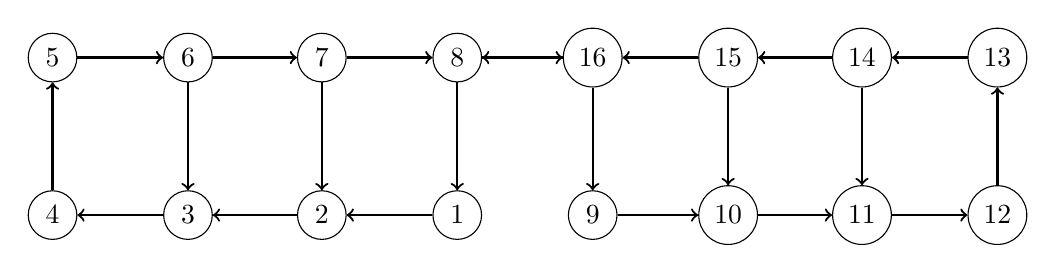
\begin{tikzpicture}[scale=2,vertex/.style={draw,circle}, arc/.style={draw,thick,->}]
        \foreach [count=\i] \coord in {(2.57,0),(1.71,0),(0.86,0),(0,0),(0,1),(0.86,1),(1.71,1),(2.57,1),(3.43,0),(4.29,0),(5.14,0),(6,0),(6,1),(5.14,1),(4.29,1),(3.43,1)}{
            \node[vertex] (p\i) at \coord {\i};
        }

        \foreach [count=\r] \row in {{0,1,0,0,0,0,0,0,0,0,0,0,0,0,0,0},{0,0,1,0,0,0,0,0,0,0,0,0,0,0,0,0},{0,0,0,1,0,0,0,0,0,0,0,0,0,0,0,0},{0,0,0,0,1,0,0,0,0,0,0,0,0,0,0,0},{0,0,0,0,0,1,0,0,0,0,0,0,0,0,0,0},{0,0,1,0,0,0,1,0,0,0,0,0,0,0,0,0},{0,1,0,0,0,0,0,1,0,0,0,0,0,0,0,0},{1,0,0,0,0,0,0,0,0,0,0,0,0,0,0,1},{0,0,0,0,0,0,0,0,0,1,0,0,0,0,0,0},{0,0,0,0,0,0,0,0,0,0,1,0,0,0,0,0},{0,0,0,0,0,0,0,0,0,0,0,1,0,0,0,0},{0,0,0,0,0,0,0,0,0,0,0,0,1,0,0,0},{0,0,0,0,0,0,0,0,0,0,0,0,0,1,0,0},{0,0,0,0,0,0,0,0,0,0,1,0,0,0,1,0},{0,0,0,0,0,0,0,0,0,1,0,0,0,0,0,1},{0,0,0,0,0,0,0,1,1,0,0,0,0,0,0,0}}{
            \foreach [count=\c] \cell in \row{
                \ifnum\cell=1%
                    \draw[arc] (p\r) edge (p\c);
                \fi
            }
        }
    \end{tikzpicture}
  \end{center}
  It is easy to see the exponential nature of this graph. However, we are going to flip a couple of the edges to make the analysis easier.
  \begin{center}
    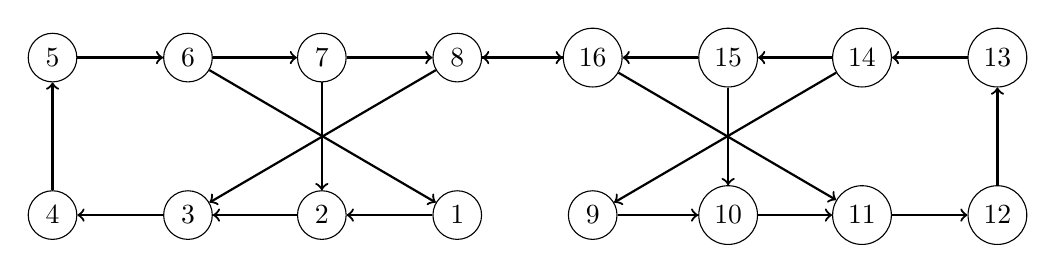
\begin{tikzpicture}[scale=2,vertex/.style={draw,circle}, arc/.style={draw,thick,->}]
        \foreach [count=\i] \coord in {(2.57,0),(1.71,0),(0.86,0),(0,0),(0,1),(0.86,1),(1.71,1),(2.57,1),(3.43,0),(4.29,0),(5.14,0),(6,0),(6,1),(5.14,1),(4.29,1),(3.43,1)}{
            \node[vertex] (p\i) at \coord {\i};
        }

        \foreach [count=\r] \row in {{0,1,0,0,0,0,0,0,0,0,0,0,0,0,0,0},{0,0,1,0,0,0,0,0,0,0,0,0,0,0,0,0},{0,0,0,1,0,0,0,0,0,0,0,0,0,0,0,0},{0,0,0,0,1,0,0,0,0,0,0,0,0,0,0,0},{0,0,0,0,0,1,0,0,0,0,0,0,0,0,0,0},{1,0,0,0,0,0,1,0,0,0,0,0,0,0,0,0},{0,1,0,0,0,0,0,1,0,0,0,0,0,0,0,0},{0,0,1,0,0,0,0,0,0,0,0,0,0,0,0,1},{0,0,0,0,0,0,0,0,0,1,0,0,0,0,0,0},{0,0,0,0,0,0,0,0,0,0,1,0,0,0,0,0},{0,0,0,0,0,0,0,0,0,0,0,1,0,0,0,0},{0,0,0,0,0,0,0,0,0,0,0,0,1,0,0,0},{0,0,0,0,0,0,0,0,0,0,0,0,0,1,0,0},{0,0,0,0,0,0,0,0,1,0,0,0,0,0,1,0},{0,0,0,0,0,0,0,0,0,1,0,0,0,0,0,1},{0,0,0,0,0,0,0,1,0,0,1,0,0,0,0,0}}{
            \foreach [count=\c] \cell in \row{
                \ifnum\cell=1%
                    \draw[arc] (p\r) edge (p\c);
                \fi
            }
        }
    \end{tikzpicture}
  \end{center}
  Where each edge either has probability 1 or 1/2 depending on the number of outgoing edges. Now let's assume the worst case where all the mass is located at node 1. Then the mass will move to node 6. However, at this step, half the mass will only continue forward. Thus, only 1/8 makes it across the bridge. In the general setting, we're going to have the probability of crossing the bridge being $\frac{1}{2^{n/4-1}}$. Now, the process restarts but with mass $1-\frac{1}{2^{n/4-1}}$ at node 3. One last thing to note is that each loop forces the mass to move $n/2$ nodes. Thus, the expected time for half the mass to cross the bridge is going to be the solution of the first $i$ such that
  \begin{gather*}
    \sum_{i} \frac{1}{2^{n/4-1}} \cdot m_i \cdot \frac{n}{2} \geq 1/2
  \end{gather*}
  where $m_i$ is the mass on the $i^{th}$ loop $(1-\frac{1}{2^{n/4-1}}) \cdot m_{i-1}$. From this,
  \begin{gather*}
    \sum_{i} \frac{1}{2^{n/4-1}} \cdot m_i \cdot \frac{n}{2} = \frac{n}{2^{n/4}} \sum_{i} m_i \\
    \leq \frac{n}{2^{n/4}} \sum_{i} 1 = \frac{n}{2^{n/4}} i
  \end{gather*}

  From here, it is clear that $i$ is exponential in $n$.
\end{answer}

\clearpage

\begin{exercise}
  Describe an example (i.e., an appropriate set of $n$ points in $\mathbb{R}^n$) that shows that the Johnson-Lindenstrauss dimension reduction method - the transformation described in Lecture, with appropriate scaling - does \textit{not} preserve $\ell_1$ distances within even factor 2. (Extra credit: Show that no \textit{linear transformation} suffices, let alone J-L).
\end{exercise}

\begin{answer}
  We use the following vectors in $\mathbb{n}$,
  \begin{gather*}
    e_1 = (1,0,0,\mathellipsis,0) \\
    -e_1 = (-1,0,0,\mathellipsis,0) \\
    e_2 = (0,1,0,\mathellipsis,0)
  \end{gather*}
  Notice that the $\ell_1$ distances between these vectors are all 2. Now we'll randomly draw $m$ independent vectors from a distribution on $\{ -\frac{1}{m}, \frac{1}{m} \}^n$. Using these vectors for the projection, we will have $\pi(e_1) = -\pi(-e_1)$ by linearity. We will also have the projection $\pi(e_2)$  be a random vector with entries in $\{ -\frac{1}{m}, \frac{1}{m} \}$ dues to choice of random vectors. But, this will agree with one of $e_1$ or $-e_1$ on more than half of the coordinates. Thus, the $\ell_1$ distance between $\pi(e_2)$ and $\pi(e_1)$ or $\pi(-e_1)$ will be $< 1$ and hence not even a factor of 2 within the original distance.
\end{answer}

\clearpage

\begin{exercise}
  (Dimension reduction for SVM's with margin) Suppose we are given two sets $P$, $N$ of unit vectors in $\mathbb{R}^n$ with the guarantee that there exists a hyperplane $a \cdot x = 0$ such that every point in $P$ is on one side and every point in $N$ is on the other. Furthermore, the $\ell_2$ distance of each point $P$ and $N$ to this hyperplane is at least $\epsilon$. Then show using the Johnson Lindenstrauss lemma (hint: you can use it as a black box) that a random linear mapping to $O(\log n/\epsilon^2)$ dimensions and such that the points are still separable by a hyperplane with margin $\epsilon/2$.
\end{exercise}

\begin{answer}
  We first define the set of points $P = \{p_i\}$ and $N = \{n_i\}$. We then add more points to make the analysis easier. $a-P = {a-p_i}$, $a-N = \{a-n_i\}$, $\{0\}$, and $\{a\}$. Recall that all $p_i$, $n_i$ are unit vectors and we can choose $a$ to be aswell. We then apply J-L to the union of all these sets so that the distortion is at most $\epsilon$. Call this J-L projection $\pi(\cdot)$. Thus the new margin is,
  \begin{gather*}
    \pi(p_i) \cdot \pi (a) = \frac{1}{2} \left( \lvert \pi(p_i) \rvert^2 + \lvert \pi(a) \rvert^2 - \lvert \pi(p_i) -\pi(a) \rvert^2 \right) \\
    \geq \frac{1}{2}(1 - \epsilon)\lvert p_i \rvert^2 + \frac{1}{2}(1 - \epsilon)\lvert a \rvert^2 - \frac{1}{2}(1 - \epsilon)\lvert a - p_i \rvert^2 \\
    = (1 - \epsilon) - \frac{1}{2}(1 - \epsilon)\lvert a - p_i \rvert^2 \\
    = (1-\epsilon)(1 - \frac{1}{2}\lvert a - p_i \rvert^2) \\
    = (1-\epsilon)(1-\epsilon/2)
  \end{gather*}
  Where we used the fact that $a \cdot b = 1/2(a^2 + b^2 -(a+b)^2)$ in the first line. Then the definition of the J-L projection. Which shows that the margin is $\epsilon/2$.
\end{answer}

\clearpage

\begin{exercise}
  Recall that $G(n,1/2)$ is the random graph on $n$ nodes in which each edge is present with probability exactly $1/2$. In the planted clique problem, you are given a graph $G \sim G(n,1/2)$ with a clique ``planted'' on some $k$ special vertices. In a previous homework, you showed that with high probability, $G \sim G(n,1/2)$ contains no clique of size more than $2 \log (n)$ thus, if $k \gg 2 \log (n)$, the added clique is the unique maximum clique in $G$. In this question, we explore a spectral algorithm for the planted clique problem.

  \begin{enumerate}[label=\alph*)]
    \item Show that the second largest eigenvalue of the adjancency matrix of $G \sim G(n,1/2)$ is at most $O(\sqrt{n})$ with high probability. (Hint: Use the method from the class that bounds the largest eigenvalue of a random matrix).
    \item Show that the second largest eigenvalue of the adjancency matrix of $G(n,1/2)$ + $k$-clique is at least $k/2$ whenever $k > 4\sqrt{n}$.
    \item Use a) and b) to give an algorithm that with high probability correctly detects whether a $k$-clique has been added to a random graph for $k > 4\sqrt{n}$. Use matlab, scipy, or any other package to compute the eigenvalues of $G(n,1/2)$ and $G(n,1/2)$ + $k$-clique for $n = 400, 800, 1200$ and $k \in [\sqrt{n}/4, 4\sqrt{n}]$. Include a table with the top 3 eigenvalues. (Do 3 repetitions with newly sampled graphs for each $n$ to see if the eigenvalue distribution is pretty stable over samples). Report your results. Do they agree with the calculations made in a) and b).
    \item (Extra Credit) Can you recover the vertices of the added clique from the second eigenvector of $G \sim G(n,1/2)$ + $k$-clique for $k$ above?
  \end{enumerate}
\end{exercise}

\begin{answer}
  \leavevmode
  \begin{enumerate}[label=\alph*)]
    \item We apply Theorem 4 of lecture notes 12 that stipulates exactly this condition. Thus, if we let $A' = A - \frac{1}{2} 1^T \cdot 1$ we get that $E[A_{ij}] = 0$ and the random variables are in $[-1,1]$ then the largest eigenvalue of the this new random adjancency matrix is at most $O(\sigma \sqrt{n})$ where $\sigma$ is the variance of the Bernoulli random variable (-1/2,1/2). This implies that the second largest eigenvalue of $A$ is on the order of $O(\sqrt{n})$.

    \item  Let $A$ be the adjacency matrix for the planted clique graph. F irst, we write the ones vector $1 = v + s$ where $v$ is the parallel vector to the largest eigenvector of $A$ and $s$ is the orthogonal part. We will show a bound on the norm of $s$.

    We denote the vector $d$ to be the vector whose $i^{it}$ entry is the degree of the vertex $i$. Then, $A \cdot 1 = d$ which is equivalent to $A(v+s) = \lambda_1 v + As$. We now subtract $n/2$ from both sides to get
    \begin{gather*}
      d - (n/2) \cdot 1 = (\lambda - n/2)v + (A - (n/2)I)s
    \end{gather*}
    Taking the norm of both sides, the cross terms are 0 since $s$ and $v$ are orthogonal,
    \begin{gather*}
      \sum_{i=1}^n (d_i -n/2)^2 = (\lambda_1 - n/2)^2 \lVert v \rVert^2 + \lVert (A - (n/2)I) s \rVert
    \end{gather*}
    Using Theorem 4 to bound the eigenvalues  of $(A - (n/2)I)$ and Fermi's gracious ``main ideas'' we get
    \begin{gather*}
      \lVert (A - (n/2)I) s \rVert > \lVert s \rVert (n/2 - k -2 \sqrt{n})
    \end{gather*}
    Which yields
    \begin{gather*}
      \lVert s \rVert^2 \leq 5 + 5k^3/n^2
    \end{gather*}
    After bounding $\sum_{i=1}^n (d_i -n/2)^2 = \sum_{i=1}^n d_i^2 - d_i n + n^2/4 \leq \sum_{i=1}^n k^2 + n^2 \leq k^3 + n^2$ with high probability.

    We now use Courant-Fischer to write $\lambda_2$ as the largest eigenvalue of
    \begin{gather*}
      A' = A - \lambda_1 \frac{v v^T}{\lVert v \rVert^2}
    \end{gather*}

    Now let $1_k$ be the indicator of the $k$-clique indices of the graph.
    \begin{gather*}
      \lambda_2 \leq \frac{1_k^T A' 1_k}{k} = \frac{1_k^T A 1_k - 1_k^T \lambda_1 \frac{v v^T}{\lVert v \rVert^2} 1_k}{k} \\
      = \frac{1_k^T A 1_k - \lambda_1 \frac{\langle 1_k, v \rangle^2}{\lVert v \rVert^2}}{k}
    \end{gather*}

    Since $1_k$ is the indicator, then $1_k^T A 1_k$ counts the $k$-clique twice iteratively so it equals $k^2$. We will also replace $v = 1 - s$.
    \begin{gather*}
      = \frac{k^2 - \lambda_1 \frac{\langle 1_k, 1-s \rangle^2}{\lVert 1-s \rVert^2}}{k}
    \end{gather*}

    Going further requires one to use the bound on $\lambda_1$ found in the first question. That is, $\lambda_1 \leq \sqrt{n}$. Another bound to use would be $\lVert 1-s \rVert^2 = 1^T 1 - 2 s^T 1 + \lVert s \rVert^2 \leq n - s^T 1 + 5 + 5k^3/n^2 = O(k^3/n^2)$.

    \item The algorithm goes as follows. Step 1) find the second largest eigenvector of the adjacency matrix $G$. 2) Pick the $k$ indices with the largest values in the eigenvector. Denote this set of indices as $V$. Then pick all the vertices in $G$ that have at least $3k/4$ neighbours in $V$. This algorithm was developed by Alon, Krivelevich, and Sudakov in their paper ``Finding a large hidden clique in a random graph''. This paper also contains similar proofs to the previous parts. My results for the simulation are below. As you can see, the first eigenvalue is roughly $n/2$. As well, when you approach $4\sqrt{n}$, the second eigenvalue begins to get bounded by $k/2$.

    For $n=400$:
    \begin{center}
      \begin{tabular}{ | c | c | c | c | c | c | c | c | c |}
        \hline
        Eigenvalue & no $k$ & $\sqrt{n}/4$ & $\sqrt{n}/3$ & $\sqrt{n}/2$ & $\sqrt{n}$ & $\sqrt{n}*2$ & $\sqrt{n}*3$ & $\sqrt{n}*4$ \\
        \hline
        $1^{st}$ & 200.31 & 200.35 & 200.41 & 200.54 & 201.21 & 204.71 & 210.38 & 218.22 \\
        $2^{nd}$ & 19.02 & 19.02 & 19.03 & 19.02 & 19.03 & 20.98 & 23.34 & 25.39 \\
        $3^{rd}$ & 18.70 & 18.71 & 18.71 & 18.78 & 28.99 & 18.95 & 18.77 & 18.51 \\
        \hline
      \end{tabular}
    \end{center}

    For $n=800$:
    \begin{center}
      \begin{tabular}{ | c | c | c | c | c | c | c | c | c |}
        \hline
        Eigenvalue & no $k$ & $\sqrt{n}/4$ & $\sqrt{n}/3$ & $\sqrt{n}/2$ & $\sqrt{n}$ & $\sqrt{n}*2$ & $\sqrt{n}*3$ & $\sqrt{n}*4$ \\
        \hline
        $1^{st}$ & 399.43 & 399.50 & 399.54 & 399.72 & 400.54 & 403.68 & 409.09 & 417.28 \\
        $2^{nd}$ & 27.36 & 27.35 & 27.37 & 27.34 & 27.38 & 32.14 & 39.17 & 44.25 \\
        $3^{rd}$ & 27.24 & 27.25 & 27.25 & 27.27 & 27.22 & 27.33 & 27.04 & 26.88 \\
        \hline
      \end{tabular}
    \end{center}

    For $n=1200$:
    \begin{center}
      \begin{tabular}{ | c | c | c | c | c | c | c | c | c |}
        \hline
        Eigenvalue & no $k$ & $\sqrt{n}/4$ & $\sqrt{n}/3$ & $\sqrt{n}/2$ & $\sqrt{n}$ & $\sqrt{n}*2$ & $\sqrt{n}*3$ & $\sqrt{n}*4$ \\
        \hline
        $1^{st}$ & 598.33 & 598.40 & 598.46 & 598.63 & 599.38 & 602.63 & 608.11 & 615.95 \\
        $2^{nd}$ & 33.96 & 33.95 & 33.96 & 33.98 & 34.20 & 40.40 & 49.19 & 58.04 \\
        $3^{rd}$ & 33.87 & 33.82 & 33.84 & 33.89 & 33.82 & 33.78 & 33.73 & 33.46 \\
        \hline
      \end{tabular}
    \end{center}

    \begin{lstlisting}[style=Matlab-editor, basicstyle=\scriptsize]
      clear;
      clc;

      n = 1200;
      p = 0.5;

      % generate graph
      A = rand(n,n) < p;
      A = triu(A,1);
      A = A + A';

      [V,D] = eig(A);
      results(1,1) = D(n-2,n-2)
      results(1,2) = D(n-1,n-1)
      results(1,3) = D(n,n)

      % clique is matrix of all ones
      k = ceil(sqrt(n)/4);
      K = ones(k);

      % index of clique to the top right corner
      i = 1;
      j = n;
      % insert clique
      A(i:i+k-1, j-k+1:n) = K;
      A = triu(A,1);
      A = A + A';

      [V,D] = eig(A);
    \end{lstlisting}

    \item skipped.

  \end{enumerate}
\end{answer}

\clearpage

\begin{exercise}
  Implement the portfolio management appearing in the notes for Lecture 13 (``Going with the Slope: Offline, Online and Randomly'') in any programming environment and check its performance on S\&P stock data (download from http://ocobook.cs.princeton.edu/links.htm). Include your code as well as the final performance (i.e., the percentage gain achieved by your strategy).
\end{exercise}

\begin{answer}
  The code done for the simulation is below. I got that the CRP yielded a loss of 7.18\% which is right in line with the losses that the S\&P 500 endured around that time. From 2001 to 2005, the market experienced steady decline before a slight uptick in 2004. Thus CRP would have been a bad choice at this time as you would continuously be buying losers before their up potential was realized in mid 2000's.

  \begin{lstlisting}[style=Matlab-editor, basicstyle=\scriptsize]
    clear;
    clc;

    load('data_490_1000.mat')

    % relative price vector
    r = zeros(490,1);
    wealth = 1000;
    distribution = ones(490,1)/490;
    portfolio = wealth * distribution;

    % loop over the trading days
    for i=2:1000
        % loop over stocks
        for j=1:490
            r(j) = A(j, i)/A(j,i-1);
        end
        wealth = r'*portfolio;
        portfolio = wealth * distribution;
    end
  \end{lstlisting}
\end{answer}

\clearpage

\begin{exercise}
  (Extra Credit) Calculate the eigenvectors and eigenvalues of the $n$-dimensional boolean hypercube, which is the graph with vertex set $\{-1,1\}^n$ and $x,y$ are connected by and edge iff they differ in exactly one of the $n$ locations. (Hint: Use symmetry extensively).
\end{exercise}

\begin{answer}
  Let us denote the adjacency matrix of the $n^{th}$ dimensional hypercube by $H_n$. Thus, $H_1$ is a single point and $H_2$ is the square. Writing out the first couple of matrices yields
  \begin{gather*}
    H_1 = \begin{bmatrix}
     0 & 1 \\
     1 & 0
    \end{bmatrix}, H_2 = \begin{bmatrix}
     0 & 1 & 1 & 0 \\
     1 & 0 & 0 & 1 \\
     1 & 0 & 0 & 1 \\
     0 & 1 & 1 & 0
    \end{bmatrix}, H_3 = \begin{bmatrix}
     0 & 1 & 1 & 0 & 1 & 0 & 0 & 0 \\
     1 & 0 & 0 & 1 & 0 & 1 & 0 & 0 \\
     1 & 0 & 0 & 1 & 0 & 0 & 1 & 0 \\
     0 & 1 & 1 & 0 & 0 & 0 & 0 & 1 \\
     1 & 0 & 0 & 0 & 0 & 1 & 1 & 0 \\
     0 & 1 & 0 & 0 & 1 & 0 & 0 & 1 \\
     0 & 0 & 1 & 0 & 1 & 0 & 0 & 1 \\
     0 & 0 & 0 & 1 & 0 & 1 & 1 & 0
    \end{bmatrix}
  \end{gather*}
  For recursive reasons, we'll define $H_0 = \begin{bmatrix}0\end{bmatrix}$. Then one can see that we have the recursion,
  \begin{gather*}
    H_{n+1} = \begin{bmatrix}
      H_n & I_{2^{n-1}} \\
      I_{2^{n-1}} & H_n
    \end{bmatrix}
  \end{gather*}
  Where $H_{n+1}$ is of dimenson $2^n \times 2^n$ and $H_0$ as before. Now we begin wuth out inductive hypthesis. That is, eigenvalues take the values $\{-n, -n+2, -n+4, \mathellipsis, n-4, n-2, n\}$ where the $k^{th}$ value has multiplicity $\binom{n}{k}$. This obviously works for $H_0$. The eigenvalue is $\{0\}$ and has multiplicity 1 ($\binom{0}{0}$). The eigenvector is 1.

  Now for the inductive step. Assume its true for $H_n$. Then let $\mu$ be an eigenvector for $H_n$. Then the following are both eigenvectors for $H_{n+1}$
  \begin{gather*}
    \mu_1 = \begin{bmatrix}
      \mu \\
      \mu
    \end{bmatrix} \text{ and } \mu_2 =
    \begin{bmatrix}
      \mu \\
      -\mu
    \end{bmatrix}
  \end{gather*}

  Quickly verifying,

  \begin{gather*}
    H_n \mu_1 = \begin{bmatrix}
      A_n \mu + \mu \\
      \mu + A_n \mu
    \end{bmatrix}  =
    \begin{bmatrix}
      \lambda \mu + \mu \\
      \lambda \mu + \mu
    \end{bmatrix} = (1+\lambda)
    \begin{bmatrix}
      \mu \\
      \mu
    \end{bmatrix} = (1+\lambda)\mu_1
  \end{gather*}
  Likewise,
  \begin{gather*}
    H_n \mu_2 = \begin{bmatrix}
      A_n \mu - \mu \\
      \mu - A_n \mu
    \end{bmatrix}  =
    \begin{bmatrix}
      \lambda \mu - \mu \\
      -\lambda \mu + \mu
    \end{bmatrix} = (\lambda-1)
    \begin{bmatrix}
      \mu \\
      -\mu
    \end{bmatrix} = (\lambda-1)\mu_2
  \end{gather*}
  Thus if $\mu$ is en eigenvector with eigenvalue $\lambda$ for $H_n$ then $\mu_1$ has eigenvalue $1+\lambda$ and $\mu_2$ has eigenvalue $\lambda-1$ for $H_{n+1}$. Now notice that this creates a cascading effect of $\pm 1$ for eigenvalues. This exactly recreates the structure in the inductive hypothesis. Furthermore, the multiplicities follow the exact coefficients as Pascal's triangle. That is, $\binom{n}{k}$.

  We use this recursive structure to show the eigenvalues for $H_1$ and $H_2$ for the benefit of the reader. Recall, $H_0$ is $\mu = [1]$ and $\lambda = 0$. Thus,

  \begin{gather*}
    H_1: \mu_1 = \begin{bmatrix} 1 \\ 1 \end{bmatrix}, \mu_2 = \begin{bmatrix} 1 \\ -1 \end{bmatrix} \text{ and } \lambda_1 = 1, \lambda_2 = -1 \\
    H_2: \mu_1 = \begin{bmatrix} 1 \\ 1 \\ 1 \\ 1 \end{bmatrix}, \mu_2 = \begin{bmatrix} 1 \\ 1 \\ -1 \\ -1 \end{bmatrix}, \mu_3 = \begin{bmatrix} 1 \\ -1 \\ 1 \\ -1 \end{bmatrix}, \mu_4 = \begin{bmatrix} 1 \\ -1 \\ -1 \\ 1 \end{bmatrix} \\
    \text{ and } \lambda_1 = 2, \lambda_2 = 0, \lambda_3 = 0, \lambda_4 = -2
  \end{gather*}
\end{answer}

\end{document}